%% Two-column preprint of the SQE paper (arXiv version).
%% [preprint] shows the author block; remove the option for an anonymous
%% review copy, or use [accepted] for camera-ready.
\documentclass{article}
\usepackage[T1]{fontenc}
\usepackage{microtype}
\usepackage{graphicx}
\usepackage{subcaption}
\usepackage{booktabs}
\usepackage{hyperref}
\newcommand{\theHalgorithm}{\arabic{algorithm}}
\usepackage[preprint]{sqe-preprint}
\usepackage{amsmath}
\usepackage{amssymb}
\usepackage{mathtools}
\usepackage{algorithm}
\usepackage{algorithmic}
\usepackage[capitalize,noabbrev]{cleveref}
\usepackage{xcolor}

\graphicspath{{figures/}}
% Tables are shared with the single-column build so numbers never diverge.
\newcommand{\tbl}[1]{\input{../tables/#1}}
\newcommand{\sqe}{\textsc{SQE}}

\pptitlerunning{Selective Query-Side Expansion for Agent Memory Retrieval}
% Set PDF metadata explicitly so it describes this paper.
\AtBeginDocument{\hypersetup{pdfsubject={Information Retrieval}, pdfkeywords={retrieval, query expansion, agent memory}}}

\begin{document}

\twocolumn[
  \pptitle{When Does Query Expansion Help Agent Memory?\\
    A Multi-Seed Study of Selective Expansion and Gate Reliability}

  \ppsetsymbol{equal}{*}
  \begin{ppauthorlist}
    \ppauthor{Salomon Diei}{kt}
  \end{ppauthorlist}
  \ppaffiliation{kt}{School of Computer Science and Engineering, KOREATECH, Cheonan, Republic of Korea}
  \ppcorrespondingauthor{Salomon Diei}{salomon@koreatech.ac.kr}
  \ppkeywords{retrieval, query expansion, agent memory, software engineering agents, negative results}

  \vskip 0.3in
]

\printAffiliationsAndNotice{}

\begin{abstract}
Long-horizon software agents store execution traces and later retrieve them
with natural-language questions, so the query and the memory are written in
different ``languages''. LLM query expansion can bridge this gap, but it costs
generation on every query. We study \emph{Selective Query-Side Expansion}
(\sqe{}), which expands a query with hypothetical execution traces and
paraphrases only when the top-1 dense retrieval score is low, then fuses all
rankings with Reciprocal Rank Fusion. Across 8 resampled memory stores with
rebuilt indices (4,000 queries over SWE-smith agent steps), \sqe{} reaches
69.4\% Recall@5 while expanding 48\% of queries; in a token-measured rerun it
uses 55\% fewer LLM tokens than always-on expansion. However, its gain over plain dense retrieval is small
($+0.9$ points, 95\% CI $[+0.1, +1.7]$), Recall@1 drops, and it is
statistically indistinguishable from a \emph{random} gate at the same budget.
An oracle analysis explains why: expansion helps only 5.3\% of queries and
hurts 4.2\%, so even a perfect gate gains at most 5.3 points. We release all
memory stores, per-method summaries, and verification scripts, and argue that
confidence gating, not expansion itself, is the open problem.
\end{abstract}

\section{Introduction}
\label{sec:intro}

Software-engineering agents accumulate long trajectories of observations,
commands, file edits, tests, and error traces. These records are valuable only
if a later agent can retrieve the relevant fragment when it faces a related
problem. Retrieval is hard here because queries and memories are written in
different registers: a stored memory may be a traceback or a patch diff, while
the later query asks, for example, how an off-by-one line-number bug was fixed.

Query expansion is a natural remedy. HyDE~\cite{gao2023hyde} generates a
hypothetical document and retrieves with it; for agents, the analogous unit is a
hypothetical \emph{execution trace}. Expansion is expensive, though: each
expanded query costs several LLM calls and seconds of latency. A practical
system should expand only when retrieval is likely to fail. This raises the
question we study:

\begin{center}
\emph{Can a cheap confidence signal decide which agent-memory\\queries are worth expanding?}
\end{center}

We implement \sqe{} (\cref{fig:overview}), which uses the top-1 dense score as
that signal, and evaluate it with an executed random-gate control at matched
budget, eight resampled memory stores with rebuilt indices, measured token costs, and
an oracle-gate upper bound. Our findings are mostly negative, and we think they
are useful precisely because they are negative.

\begin{figure*}[t]
  \centering
  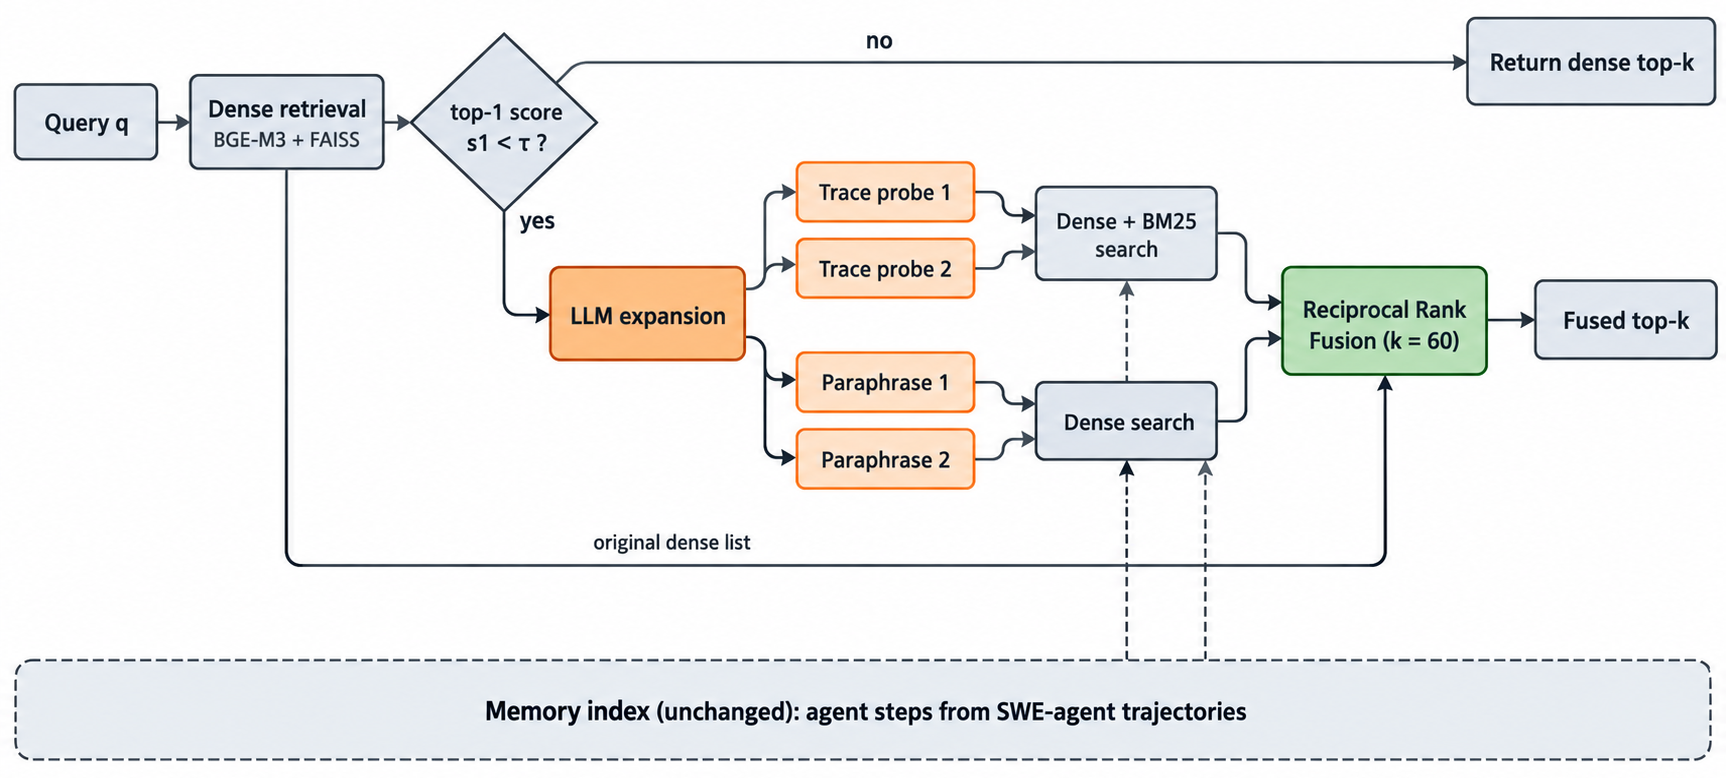
\includegraphics[width=0.92\textwidth]{method_overview.png}
  \caption{\sqe{} retrieval flow. Dense retrieval runs first; confident queries
  return the dense list unchanged. Queries whose top-1 score falls below $\tau$
  are expanded into two hypothetical trace probes (searched with dense and BM25)
  and two paraphrases (searched with dense only), all against the same unchanged
  index. The original dense list and the five probe lists are fused with RRF.}
  \label{fig:overview}
\end{figure*}

\paragraph{Contributions.}
\begin{enumerate}
  \item We formulate the trace--query mismatch in long-horizon software-agent
  memory and a selective, query-side-only expansion method that leaves the
  memory store and indices untouched (\cref{sec:method}).
  \item We run a controlled multi-seed study with an \emph{executed}
  random-gating baseline at matched expansion rate and provider-measured token
  costs (\cref{sec:results}).
  \item We show that the top-1-score gate is not better than random, and use an
  oracle-gate analysis to bound what any gate could achieve in this setting
  (\cref{sec:gate}).
  \item We release seeds, summaries, paired tests, and verification scripts so
  that every number in this paper can be recomputed (\cref{sec:repro}).
\end{enumerate}

\section{Related Work}
\label{sec:related}

\paragraph{Dense and sparse retrieval.}
Dense passage retrieval maps queries and documents to a shared embedding
space~\cite{karpukhin2020dpr}; BM25 remains a strong lexical
baseline~\cite{robertson2009bm25}. Reciprocal Rank Fusion combines ranked
lists without training a ranker~\cite{cormack2009rrf}. We keep both indices
fixed and change only the query side.

\paragraph{Query expansion with generated text.}
HyDE embeds a generated hypothetical document for zero-shot dense
retrieval~\cite{gao2023hyde}. EAR expands and reranks candidate
queries~\cite{chuang2023ear}, and HyQE ranks contexts with hypothetical query
embeddings~\cite{zhou2024hyqe}. Later analysis shows that hypothetical-document
gains can partly reflect knowledge leakage from the generator~\cite{yoon2025hypothetical}.
\sqe{} differs in its expansion unit (execution traces) and its explicit
generation gate; our results suggest the gate is the weakest component.

\paragraph{Agent memory and software agents.}
AMA-Bench and MemoryAgentBench evaluate memory over long-horizon and incremental
multi-turn interaction~\cite{zhao2026amabench,hu2025memae}. SWE-bench measures
whether an agent resolves real issues~\cite{jimenez2024swebench}, and SWE-smith
provides large-scale agent trajectories~\cite{yang2025swesmith}. Our benchmark
is narrower: retrieval of a known target episode, which we treat as an
intermediate signal rather than a substitute for task success.

\section{Method}
\label{sec:method}

Let $M=\{m_i\}_{i=1}^{N}$ be a store of execution traces. For a query $q$,
dense retrieval returns a ranked list $R_d(q)$ with top-1 cosine score
$s_1(q)$. \sqe{} expands $q$ iff $s_1(q)<\tau$; otherwise it returns $R_d(q)$
unchanged. An expanded query yields $K$ hypothetical traces and $P$ paraphrases
from an LLM. Each trace is searched with both the dense and the BM25 index,
because traces share exact identifiers with stored steps; each paraphrase is
searched with the dense index only. The original list and the $2K+P$ probe lists
(each truncated to its top 20) are fused with
\begin{equation}
  \mathrm{score}(m)=\sum_{j}\frac{1}{k+\mathrm{rank}_j(m)}.
\end{equation}
We use $\tau=0.65$, $K=P=2$, and $k=60$ throughout. The generated traces are
retrieval probes, not claims that those executions occurred.
\Cref{alg:sqe} summarizes the procedure.

\begin{algorithm}[t]
  \caption{Selective Query-Side Expansion}
  \label{alg:sqe}
  \begin{algorithmic}
    \STATE {\bfseries Input:} query $q$, threshold $\tau$, LLM $G$, budgets $K,P$
    \STATE $R_d, s_1 \leftarrow \textsc{Dense}(q)$
    \IF{$s_1 \ge \tau$}
      \STATE {\bfseries return} $R_d$
    \ENDIF
    \STATE $\mathcal{T} \leftarrow G_{\text{trace}}(q,K)$, $\;\mathcal{P} \leftarrow G_{\text{para}}(q,P)$
    \STATE $\mathcal{L} \leftarrow \{R_d\} \cup \{\textsc{Dense}(p) : p \in \mathcal{P}\}$
    \STATE $\mathcal{L} \leftarrow \mathcal{L} \cup \{\textsc{Dense}(t), \textsc{BM25}(t) : t \in \mathcal{T}\}$
    \STATE {\bfseries return} $\textsc{RRF}(\mathcal{L}, k)$
  \end{algorithmic}
\end{algorithm}

\section{Experimental Setup}
\label{sec:setup}

\paragraph{Data.} We use the \texttt{tool} split of the SWE-smith
trajectories~\cite{yang2025swesmith}, produced with SWE-agent and Claude~3.7
Sonnet. Each trajectory is cut into single agent steps (thought, action,
observation); steps under 100 characters are dropped. A memory store holds
5,000 such steps. For each seed (42--49) we shuffle a shared pool of about
16,500 steps, take 5,000 as the store, rebuild both indices, and sample 500
evaluation targets from the store. The stores are therefore resampled, not
disjoint: two stores share about 30\% of their steps, and the 4,000 targets
contain 3,527 distinct steps. For each target, an LLM that sees the step writes
one question meant to identify it, and is told not to copy identifiers, error
codes, or variable names. Exactly one stored step counts as relevant per query,
so sibling steps from the same trajectory count as misses.

\paragraph{Models.} Dense retrieval uses BAAI/bge-m3 with FAISS; sparse
retrieval uses BM25. Expansion uses Qwen3.6-35B-A3B served with vLLM.

\paragraph{Baselines.} Dense-Only, BM25-Only, Hybrid-RRF (dense + BM25),
Paraphrases-Only and HyDE-Traces-Only (always expand with one probe type),
Always-Expand (both probe types on every query), and
\textbf{Random-Gated-Expansion}, which runs the identical expansion code but
replaces the gate with seeded random decisions at a comparable rate. The random
gate is the key control: it separates the value of \emph{expanding some
queries} from the value of \emph{choosing which ones}.

\paragraph{Metrics and inference.} We report Recall@$\{1,5,10\}$ and
provider-reported tokens and latency. Uncertainty uses paired bootstrap over
query rows. These intervals pool queries across seeds and are not corrected for
multiple comparisons, so we treat them as descriptive (\cref{sec:limits}).

\section{Results}
\label{sec:results}

\begin{table}[t]
  \caption{Retrieval over 8 resampled memory stores (mean $\pm$ std over
  seeds, \%). \sqe{} expands 48.2\% of queries on average; the random gate
  expands 45.9\%.}
  \label{tab:multiseed}
  \centering
  \small
  \resizebox{\columnwidth}{!}{\tbl{multiseed_summary}}
\end{table}

\begin{table}[t]
  \caption{Paired bootstrap of \sqe{} minus each baseline, Recall@5 points,
  pooled over 4,000 query rows. $p=0.000$ denotes $p<0.001$.}
  \label{tab:paired}
  \centering
  \small
  \resizebox{\columnwidth}{!}{\tbl{multiseed_paired_tests}}
\end{table}

\paragraph{\sqe{} is slightly better than dense retrieval at Recall@5, and worse at Recall@1.}
\Cref{tab:multiseed} shows \sqe{} at 69.4\% Recall@5 against 68.5\% for
Dense-Only. The paired difference is $+0.9$ points with 95\% CI $[+0.1,+1.7]$
(\cref{tab:paired}). At query level, \sqe{} recovers 140 targets that dense
retrieval missed but loses 105 that it found, a net gain of 35 out of 4,000
(\cref{tab:winloss}, appendix). Recall@1 falls from 45.5\% to 44.5\%: fusing
expanded lists widens the candidate set but disturbs the top position.
\Cref{fig:multiseed} shows that the seed-to-seed spread ($\pm$2.7 points) is
three times larger than the method effect.

\paragraph{The gate does not beat a random gate.}
Against Random-Gated-Expansion at a similar budget, \sqe{} gains $+0.5$
points with CI $[-0.2,+1.1]$. Against Always-Expand the difference is $+0.1$
$[-0.4,+0.7]$. Expanding about half of the queries recovers essentially all of
the benefit of expanding every query, but \emph{which} half matters little.

\paragraph{Selectivity is still a large cost saving.}
\Cref{fig:cost} plots measured tokens (seed 42 rerun) against Recall@5. \sqe{} uses 405
tokens and 2.8\,s per query versus 899 tokens and 5.4\,s for Always-Expand
(\cref{tab:tokens}, appendix), with equal Recall@5. Trace-only expansion is the
worst operating point: it is expensive and loses 4.7 points to dense retrieval,
so hypothetical traces help only when fused with paraphrases and the original
query.

\begin{figure}[t]
  \centering
  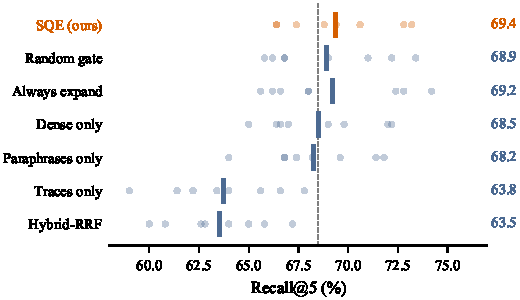
\includegraphics[width=\columnwidth]{multiseed_recall5.pdf}
  \caption{Recall@5 per seed (dots) and 8-seed mean (bar). The dashed line is
  the Dense-Only mean. Seed variance dominates every expansion effect.}
  \label{fig:multiseed}
\end{figure}

\begin{figure}[t]
  \centering
  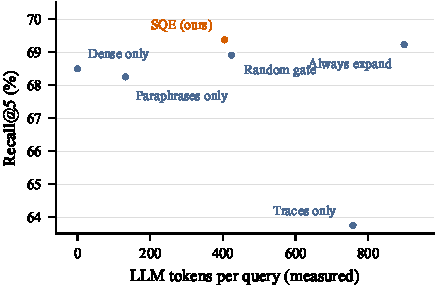
\includegraphics[width=\columnwidth]{cost_quality.pdf}
  \caption{Cost against quality. $x$: provider-measured LLM tokens per query
  (seed 42); $y$: 8-seed mean Recall@5. \sqe{} matches Always-Expand at
  roughly half the tokens, but so does the random gate.}
  \label{fig:cost}
\end{figure}

\section{Why the Gate Fails}
\label{sec:gate}

\paragraph{Low confidence marks hard queries, not fixable ones.}
On seed 42, expanded queries reach 61.7\% Recall@5 and non-expanded ones
75.9\% (\cref{tab:gatediag}, appendix). The top-1 score does find hard
queries, but expansion does not reliably repair them.

\paragraph{The threshold barely matters.}
\Cref{fig:threshold} sweeps $\tau$ on seed 42. Recall@5 stays within a
2.2-point band while the expansion rate goes from 0\% to 100\%, and the best
post-hoc threshold (0.62) beats the fixed one by only 0.8 points. Held-out
selection does not change this picture: leave-one-seed-out threshold selection
gives $+0.6$ points over dense retrieval with CI $[-0.1,+1.3]$
(\cref{tab:loso}, appendix), and BM25-agreement gate variants do
not close the gap (\cref{tab:variants}, appendix).

\paragraph{There is little headroom for any gate.}
To bound what a better gate could achieve, we combine executed Dense-Only and
Always-Expand rows on the held-out half of each seed. An oracle that expands
exactly the queries that expansion helps would reach 73.5\% Recall@5, against
68.2\% for dense retrieval (\cref{fig:headroom}). Expansion helps 5.3\% of
queries and hurts 4.2\%; the remaining 90\% have the same outcome either way.
With helpful and harmful cases this balanced and this rare, a scalar
confidence score has little signal to exploit.

\begin{figure}[t]
  \centering
  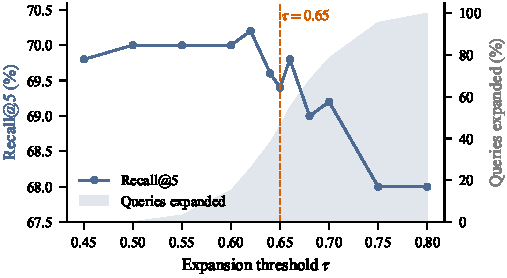
\includegraphics[width=\columnwidth]{threshold_sweep.pdf}
  \caption{Post-hoc threshold sweep on seed 42. Recall@5 (line, left axis)
  varies by about 2 points while the fraction of expanded queries (shaded,
  right axis) spans 0--100\%.}
  \label{fig:threshold}
\end{figure}

\begin{figure}[t]
  \centering
  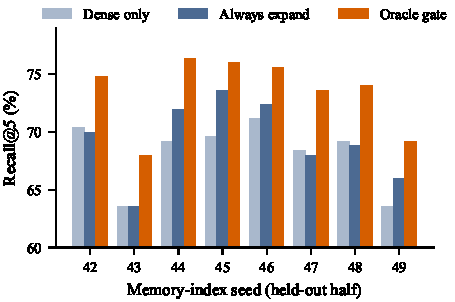
\includegraphics[width=\columnwidth]{gate_headroom.pdf}
  \caption{Held-out oracle headroom. Even a perfect per-query gate gains about
  5 points over dense retrieval; always expanding gains about 1.}
  \label{fig:headroom}
\end{figure}

\section{Limitations}
\label{sec:limits}

\paragraph{Queries.} Evaluation queries are generated by an LLM that sees the
target trace, which can leak target-specific wording and overstate
discriminability. A human-audit packet is prepared but unlabeled.

\paragraph{Relevance labels.} Only the exact source step is relevant. Adjacent
steps of the same trajectory can answer the same question, so Recall@$k$ may
understate all methods, and possibly expansion more than dense retrieval.

\paragraph{No downstream outcome.} Recall@$k$ is an intermediate signal; we do
not measure whether retrieved memories change agent Pass@1 on SWE-bench-style
tasks~\cite{jimenez2024swebench}.

\paragraph{Statistics.} Bootstrap intervals pool queries across seeds, but the
seeds share about 30\% of their memories and some targets, so the 4,000 rows
are not independent and the intervals are likely too narrow. No multiplicity
correction is applied. A confirmatory study
should pre-register one contrast and use seed- or task-clustered inference.

\paragraph{Scope.} One embedder, one generator, one trace source, and one
memory size. The upstream dataset revision was not pinned for the completed
runs, and generator inference seeds were not stored; the released sampled
stores are therefore the fixed evidence.

\section{Reproducibility}
\label{sec:repro}

Code, paper sources, and per-seed summaries are at
\url{https://github.com/Salomondiei08/sqe-experiment}; memory stores,
evaluation pairs, and result artifacts are at
\url{https://huggingface.co/datasets/TheReinventGuy/sqe-experiment}.
\texttt{scripts/07\_verify\_experiment.py} recomputes all metrics from result
files and checks that each table matches its declared source. Every figure in
this version is produced by \texttt{make\_figures.py} in the repository directly from
the released JSON, except \cref{fig:overview}, which is an illustration.
The upstream dataset revision was not pinned for the completed runs.

\section{Conclusion}
\label{sec:conclusion}

Selective query-side expansion halves the generation cost of always-on
expansion for agent-memory retrieval with no loss in Recall@5. But in our
setting the selection itself is no better than chance, the gain over dense
retrieval is under one point, and an oracle bound shows little room for any
scalar gate. We conclude that the open problem is predicting \emph{which}
queries expansion will fix, and that future work should evaluate learned gates
against random-budget controls and measure downstream agent success.

\section*{Impact Statement}
This work studies retrieval for software-engineering agents. Better memory
retrieval could make such agents more capable; we do not foresee negative
impacts beyond those of software agents generally. All data are public agent
trajectories.

\section*{Acknowledgments and Disclosure}
An earlier version of this work was presented at NAFSIK 2026. The author used
LLM-based assistance to organize the experiment package, write audit scripts,
edit text, and draw \cref{fig:overview}. All numbers come from executed result
files, and the author reviewed every claim.

\bibliography{../references}
\bibliographystyle{sqe-preprint}

\newpage
\appendix
\onecolumn

\section{Additional Results}

\begin{table}[h]
  \caption{Seed-42 results for all methods (\%). This seed carries the
  per-query rows, case analysis, and token measurements.}
  \label{tab:seed42}
  \centering
  \small
  \tbl{main_results}
\end{table}

On seed 42, \sqe{} reaches 69.4\% Recall@5 against 69.8\% for Dense-Only
($-0.4$) and 64.0\% for Hybrid-RRF ($+5.4$); Recall@1 is 47.2\% against 49.0\%.
The multi-seed aggregate in \cref{tab:multiseed} is the primary evidence.

\begin{table}[h]
  \caption{Query-level top-5 wins and losses of \sqe{} against Dense-Only.}
  \label{tab:winloss}
  \centering
  \small
  \tbl{win_loss_analysis}
\end{table}

\begin{table}[h]
  \caption{Provider-reported token usage and latency (seed 42, 500 queries,
  expansion cache disabled).}
  \label{tab:tokens}
  \centering
  \small
  \tbl{measured_token_cost}
\end{table}

\begin{table}[h]
  \caption{Seed-42 gate split by expansion decision.}
  \label{tab:gatediag}
  \centering
  \small
  \tbl{gate_diagnostics}
\end{table}

\begin{table}[h]
  \caption{Leave-one-seed-out top-1 threshold selection.}
  \label{tab:loso}
  \centering
  \small
  \tbl{cross_seed_top1_gate}
\end{table}

\begin{table}[h]
  \caption{Held-out score-only and BM25-agreement gate variants.}
  \label{tab:variants}
  \centering
  \small
  \tbl{gate_variant_diagnostics}
\end{table}

\begin{table}[h]
  \caption{Seed-42 examples where \sqe{} and Dense-Only differ at top-5.
  Illustrative only.}
  \label{tab:cases}
  \centering
  \scriptsize
  \resizebox{\textwidth}{!}{\tbl{case_analysis}}
\end{table}

\end{document}
